%
%=============================--C--=============================%
\clearpage
\subsection{2. Canal de transmiss\~ao e filtro adaptado}
\label{subsec:filtro-adaptado}
Numa situação ideal (i.e., na ausência de ruído branco), a desmodulação de um sinal digital requer a utilização de um filtro passa-baixo regular. Não obstante, em aplicações reais é necessário mitigar os efeitos da presença do ruído branco (térmico), cuja densidade espectral de potência é constante ($S_W(f)=N_0/2$). Esta característica torna o AWGN impossível de eliminar completamente. 
\\[-7em]

\begin{tabular}{C{6.5cm}  L{6.5cm}}
    \label{fig:gnuradio1}
    \raisebox{-2.1\height}{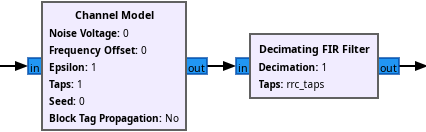
\includegraphics[width = 1\linewidth]{img/intro/channel_matchedfilter.png}}\captionof{figure}{Modelo do canal de transmissão e filtro adaptado (\textit{GNU Radio}).} & \noindent\fcolorbox{black}{white}{%
        \minipage[t]{\dimexpr\linewidth-2\fboxsep-2\fboxrule\relax}
            \textbf{Nota} $\rightarrow$ Em regime laboratorial, o canal de transmiss\~ao é simulado através do bloco \textit{Channel Model}, onde é variado o \textit{"AWGN noise level as a voltage"}\cite{channelmodel-gnuradio} de 0 a 4 V.
        \endminipage}
\end{tabular} 

Para atenuar o impacto deste ruído, utiliza-se um filtro adaptado que maximiza a relação sinal-ruído nos instantes de amostragem.

\begin{figure}[H]
    \centering
    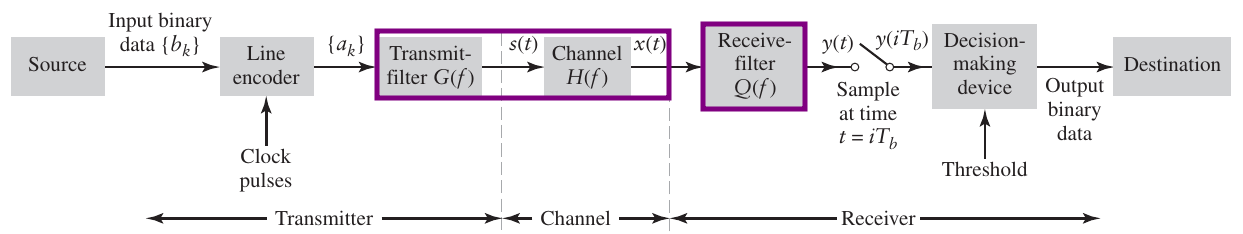
\includegraphics[width = 1\linewidth]{img/intro/filtro_adaptado1.png}
    \caption{Trasmissão e recepção com filtro adaptado.}
    \label{fig:filtro-adaptado}
\end{figure}

Tomando $G(f)H(f) \delequal P^{1/2}(f)$, temos que o filtro adaptado toma a seguinte forma: $Q(f) \delequal P^{1/2}(f)$.\footnotemark[4]

\footnotetext[4]{Sendo o sistema caracterizado por $p(t) = g(t)\ast h(t)\ast q(t) \xrightarrow{\mathcal{F}} P(f) = G(f)H(f)Q(f)$, obtém-se o sinal PAM: $y(t) = \sum\limits_{k=-\infty}^{\infty} a_k p(t-kT_b)$.}

\subsubsection{2.1 \textit{Pulse-shaping}}

\begin{quotation}
    "The most popular pulse-shaping filter seems to be the “raised-cosine” filter. It’s a good low-pass filter for limiting the bandwidth our signal will occupy, and it also has the property of summing to zero at intervals of $T_S$ [eliminar interferência intersimbólica (IIS)] (...)"\cite{pysdr}
\end{quotation}

Mediante o supracitado, e tendo em consideração o formato do sinal $y(t)$ (vide a \hyperref[fig:filtro-adaptado]{Fig. 3}), é trivialmente deduzido que para obter o formato \textit{raised cosine} e executar o processo de \textit{matched filtering} no ramo de receção (tal como no projeto corrente), recorre-se a um \textit{root raised cosine} (como apresentado na \hyperref[fig:gnuradio1]{Fig. 2}).